\section{Traditionelle Architektur einer Persistenzschicht}
Herkömmliche Enterprise-Systeme wurden in zwei Teilsysteme unterteilt. Zum einen in das OLAP(On-line Analytical Processing)- und zum anderen in das OLTP(On-line Transaction Processing)-System. In dem OLTP-system werden in Echtzeit Daten hinzugefügt, modifiziert oder gelöscht. Es entstehen also viele Transaktionen. Das OLAP-system wird verwendet um Analysen auf den Daten laufen zu lassen. Das beinhaltet zum Beispiel Anfragen, die herausfinden sollen, welches Produkt am häufigsten gekauft wurde. Entsprechend werden viele Daten gelesen und wenig geschrieben. Es entstehen also wenige Transaktionen, diese die entstehen sind jedoch komplexer.
\\
Damit die Analysen und das Geschäft auf den möglichst aktuellen Daten laufen, müssen die Daten von dem OLTP-System auf das OLAP-System überspielt werden. Diese Funktion übernimmt die Persistenzschicht. Der Prozess wird ETT (Extraction Transformation Transportation) genannt und ermöglicht die Vereinigung von Daten aus verschiedenen und meist heterogenen Quellen. Die Heterogenität muss dazu auf mehreren Ebenen (System, Schema, Daten) geregelt werden. Weil die Entscheidungen im betrieblichen Umfeld auf konsequentem Basis basieren müssen um eine effiziente Analyse zu ermöglichen, müssen Daten so transformiert werden, dass sie auf das Analysefeld bezogen in der richtigen Form zur Verfügung stehen. Einige Voraussetzungen dafür sind die Vorauswahl geeigneter Daten, die Herstellung eines Zeitbezuges und die notwendigen Aggregationen unterschiedlicher Eigenschaften.\cite{koppen2014data}
\subsection{Trennung von OLAP und OLTP}
Als OLTP und OLAP entwickelt wurden, analysierte man was die Aufgaben einer Datenbank größtenteils darstellen. Zum einen gibt es Schreiboperationen, bei denen man neue Zeilen einfügt, löscht oder vorhandene Zeilen bearbeitet. Diese Operationen betreffen jeweils nur wenige Zeilen einer Datenbank, dafür werden diese sehr häufig ausgeführt. Auf der anderen Seite möchte man die Daten analysieren um “versteckte” Informationen zu finden. An einem einfachen Beispiel: Eine Firma hat täglich Millionen von Verkäufen, die sie alle in einer Datenbank mitschreibt. Aus diesen Verkaufsdaten, möchte die Firma herausfinden, in welchem Zeitraum welches Produkt am meisten verkauft wurde, damit man so auf saisonale Anforderungen reagieren und diese vorhersagen kann. Diese Analysen führt man natürlich nicht so oft aus, diese sind jedoch dafür sehr komplexe Operationen und betreffen meist einen Großteil, wenn nicht sogar alle Zeilen einer Datenbank.
Diese beiden Fälle möchte man natürlich möglichst effizient ausführen um mögliche Kosten zu vermeiden.
\\
Zu dem Zeitpunkt war es mit dem Stand der Technik jedoch nicht möglich, ein Datenbanksystem zu erstellen, welches beide Anwendungsfälle abdeckt und diese jeweils schnell und kostengünstig durchführen kann. Deshalb entschied man sich,
die beiden Anwendungsfälle in unterschiedliche Datenbanksysteme aufzuteilen: OLAP(Data Warehouse) und OLTP(operative Systeme).
\\
Das OLTP-system muss hauptsächlich Schreiboperationen durchführen die nur wenige Zeilen der Datenbank betreffen. In diesem werden die neuen Daten eingefügt und es stellt somit den aktuellen Stand der laufenden Unternehmensprozesse da. Das OLTP basiert den Betrieb auf Multi-Access, schnelle und effektive Abfragen in die Datenbank. Die am häufigsten verwendeten Operationen sind INSERT, UPDATE und DELETE. Da die Daten direkt geändert und neue Informationen über neue Transaktionen bereitgestellt werden, wird eine effektive Schreiboperationsunterstützung erfordert. 
\\
Das OLAP-System muss hingegen meistens Leseoperationen durchführen für die Analyse der Daten. Man arbeitet dann also mit ziemlich vielen Zeilen der Datenbank, hat jedoch eine niedrige Transaktionsanzahl. Die Daten werden selten aktualisiert und die SELECT-Operation gilt als Hauptmerkmal des Systems. Daher basiert OLAP auf READ-Operationen und aggregiert alle verfügbaren Informationen.
\subsection{Vorteile und Architektur einer modernen in-memory-basierten Datenhaltung}
Aufgrund technischer Fortschritte in der heutigen Zeit, wie zum Beispiel Multicore-Prozessoren und deutlich günstigere Preise für RAM (siehe Abbildung 1),
ist es in der heutigen Zeit möglich, OLTP und OLAP Systeme zu einem zu vereinen.
Unterstützt wird diese Möglichkeit auch durch Untersuchungen, die herausgefunden haben, dass OLAP und OLTP Systeme nicht so genutzt werden, wie gedacht. Bei beiden System sind Schreiboperationen ein Großteil der Operationen. Beide Systeme haben also doch ähnlichere Aufgaben als vorher angenommen. In-Memory Systeme nutzen die heutige neue Software für maximale Effizienz aus.
\begin{figure}[ht]
  \begin{center}
  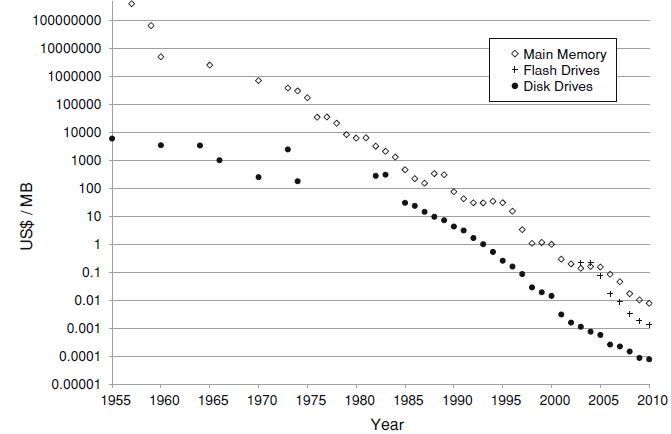
\includegraphics[width=0.5\textwidth]{images/mainflashdisk.png}
  \end{center}
  \caption{Abbildung 1: Preisentwicklung von Speichermedien (\cite{hp}S.10)}
  \label{fig_1}
\end{figure} 
\\
So werden die Daten nicht mehr in mehreren Datenbanken gespeichert, sondern nur noch im In-Memory System. Die Daten wurden bei OLTP und OLAP Systemen meist auf Festplatten oder Flash-Speicher gespeichert. Da bei In-Memory Systemen die Daten jedoch im DRAM gespeichert werden, erhält man dadurch deutlich geringere Zugriffszeiten (siehe Abbildung 2).
\\
\begin{figure}[ht]
  \begin{center}
  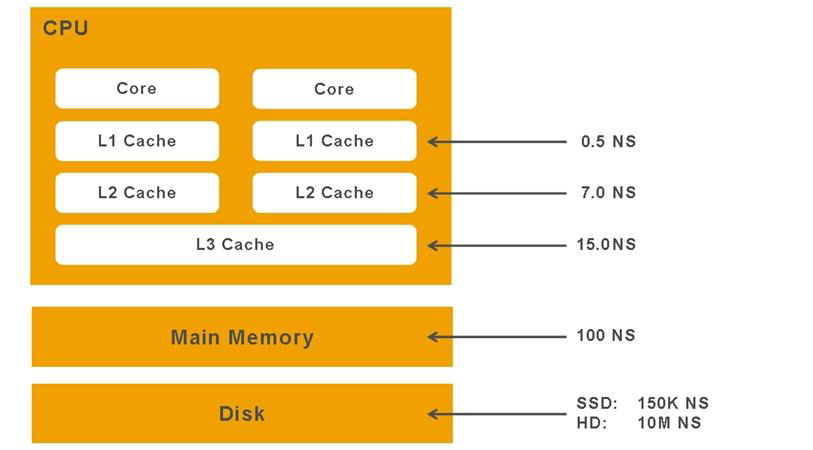
\includegraphics[width=0.5\textwidth]{images/cpu.png}
  \end{center}
  \caption{Abbildung 2: Zugriffszeiten von Speicherkompenenten (\cite{sap}S.11)}
  \label{fig_2}
\end{figure} 
Die Daten bei einem OLTP-System werden zeilenbasiert gespeichert, da man dadurch einfacher einzelne Tupel aus einer Datenbanktabelle lesen kann. Dies ist jedoch nicht sehr dafür geeignet, mehrere Einträge aus einer Spalte auszulesen.
In-Memory Systeme speichern deshalb ihre Daten spaltenbasiert (siehe Abbildung 3).
\begin{figure}[ht]
  \begin{center}
  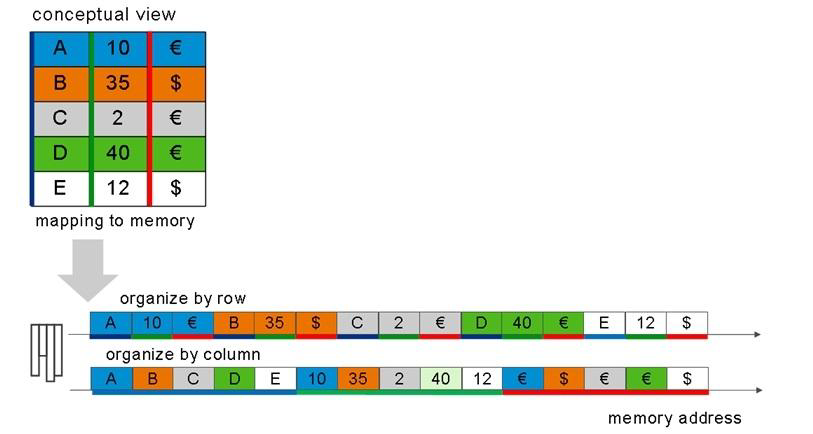
\includegraphics[width=0.5\textwidth]{images/mappingtomemory.png}
  \end{center}
  \caption{Abbildung 3: Vergleich Zeilen- und Spaltenorientierte Speicherung (\cite{sap}S.12)}
  \label{fig_3}
\end{figure} 
\\
Der Vorteil bei Spalten basierten Speicherung ist, dass bestimmte Operationen, wie zum Beispiel die Aggregation schneller ausgeführt werden können. Bei einer zeilenbasierten Speicherung kann es passieren, dass man aus jeder Zeile nur ein Wert dafür braucht, jedoch jedes Mal die gesamte Zeile einlesen muss. Bei einer spaltenbasierten Speicherung kann man jedoch einfach die gesamte Spalte dafür einlesen und muss keine unnötigen Daten in den CPU Cache laden.
Da man die gesamte Datenbank in Main Memory dauerhaft speichern will, sind die Daten auch komprimiert um diese möglichst klein zu halten.
Durch die spaltenbasierte Speicherung ist dies besonders gut möglich, da Daten von gleichen Typen jeweils zusammen gespeichert werden und es somit wahrscheinlich ist, das Werte mehrfach auftreten, da viele Spalten meist eine geringe Kardinalität Werten besitzen. Auch NULL Values oder Default Values sind meist der einzige Inhalt einer Spalte und somit komprimierbar. Dadurch kann man mit zum Beispiel einer Dictionary-Komprimierung viel Speicherplatz sparen.
Weiterhin nutzen In-Memory Systeme die Entwicklung von Multicore-CPUs aus. Die Prozesse werden dabei in kleinste Verarbeitungsschritte aufgeteilt, die jeweils dann auf mehreren Prozessoren parallel ausgeführt werden können (siehe Abbildung 4).\\
\begin{figure}[ht]
  \begin{center}
  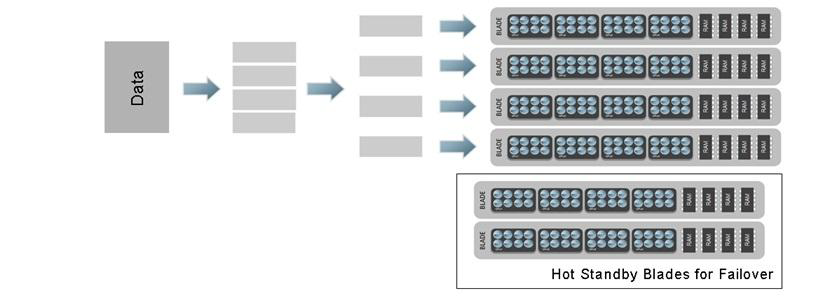
\includegraphics[width=0.5\textwidth]{images/data.png}
  \end{center}
  \caption{Abbildung 4: Daten-Verteilung bei SAP HANA (\cite{sap}S.12)}
  \label{fig_4}
\end{figure} 
All \ref{fig_1} diese Veränderungen der Architektur sorgen dafür, dass man die Daten immer 
aktuell im In-Memory System hat. Analysen werden nun immer über 
den aktuellsten Daten durchgeführt und nicht über älteren, da die Daten noch nicht vom OLTP zum OLAP System kopiert wurden. Weiterhin sind durch die geringere Zugriffszeit auf die Daten, die Parallelisierung und die Speicherung der Daten in Spaltenformat die Geschwindigkeit von Prozessen deutlich erhöht worden. Somit ist es für Nutzer der In-Memory Systeme möglich, Analysen in Echtzeit zu berechnen und vor allem die Anforderungen für die Analysen variabel ändern und es muss nicht mehr auf die Ergebnisse gewartet werden. Dadurch erledigt sich das Vorberechnen von Ergebnissen.\cite{neumannsap}
\\
